\subsection{Experiment 2: Contraction Dial Evaluation}
\label{sec:exp2_contraction}

We investigate whether targeting spectral-norm-based contraction provides a reliable ``stability dial'' for controlling unroll sensitivity.

\paragraph{Setup.}
We train models with target Lipschitz constants $L_z^* \in \{0.9, 0.95, 0.99, 0.999\}$ using spectral normalization on the update function, with 3 seeds per condition. We evaluate achieved Lipschitz constants and unroll sensitivity metrics at two projection settings: $R=10$ (default) and $R=\infty$ (projection disabled).

\paragraph{Finding 1: Dial failure.}
The spectral-norm targeting mechanism does \emph{not} produce a reliable dial. At $R=\infty$ (projection disabled), the achieved pre-projection Lipschitz constant $\hat{L}_{\text{pre}}$ varies only weakly (spread 0.064, below our 0.08 threshold) and non-monotonically across target values (Table~\ref{tab:exp2_dial_failure}). At $R=10$, projection dominates (100\% active) and post-projection Lipschitz saturates at $\approx 0.23$, masking any underlying differences.

\paragraph{Finding 2: Projection stabilizes.}
Latent-ball projection at $R=10$ provides substantial stabilization (Table~\ref{tab:exp2_projection_stabilizer}). Value stability $\Delta V$ improves from 7.7--14.8 ($R=\infty$) to 0.5--2.2 ($R=10$), approximately 6--10$\times$ reduction. Argmax agreement improves from 88--91\% to 97--99\%, a gain of 8--10 percentage points.

\begin{table}[h]
\centering
\caption{Spectral-norm dial does not control Lipschitz constant. At R=10, projection dominates (100\% active) and $\hat{L}_{post}$ saturates. At R=disabled, $\hat{L}_{pre}$ varies weakly (spread 0.064 $<$ 0.08 threshold) and non-monotonically.}
\label{tab:exp2_dial_failure}
\begin{tabular}{lcccc}
\toprule
Target $L_z$ & $\hat{L}_{pre}$ (R=$\infty$) & $\hat{L}_{post}$ (R=10) & Proj Active (R=10) & Proj Active (R=$\infty$) \\
\midrule
  0.9 & 0.473$\pm$0.002 & 0.242$\pm$0.003 & 100\% & 0\% \\
  0.95 & 0.409$\pm$0.029 & 0.219$\pm$0.005 & 100\% & 0\% \\
  0.99 & 0.448$\pm$0.016 & 0.234$\pm$0.003 & 100\% & 0\% \\
  0.999 & 0.440$\pm$0.044 & 0.231$\pm$0.010 & 100\% & 0\% \\
\midrule
  \textbf{Spread} & \textbf{0.064} & -- & -- & -- \\
\bottomrule
\end{tabular}
\end{table}

\begin{table}[h]
\centering
\caption{Projection is the primary stabilizer. R=10 projection dramatically improves stability metrics compared to disabled projection.}
\label{tab:exp2_projection_stabilizer}
\begin{tabular}{lccccc}
\toprule
Target $L_z$ & \multicolumn{2}{c}{$\Delta V$ (n=2$\to$16)} & \multicolumn{2}{c}{Argmax Agree (\%)} \\
\cmidrule(lr){2-3} \cmidrule(lr){4-5}
 & R=10 & R=$\infty$ & R=10 & R=$\infty$ \\
\midrule
  0.9 & 2.18 & 10.48 & 99.0 & 90.7 \\
  0.95 & 0.55 & 9.95 & 97.3 & 89.3 \\
  0.99 & 0.99 & 7.72 & 99.7 & 88.0 \\
  0.999 & 1.58 & 10.02 & 99.3 & 89.7 \\
\midrule
  \textbf{Mean} & \textbf{1.32} & 9.54 & \textbf{98.8} & 89.4 \\
  \textbf{Range} & [0.5, 2.2] & [7.7, 10.5] & [97, 100] & [88, 91] \\
\bottomrule
\end{tabular}
\end{table}

\begin{figure}[h]
    \centering
    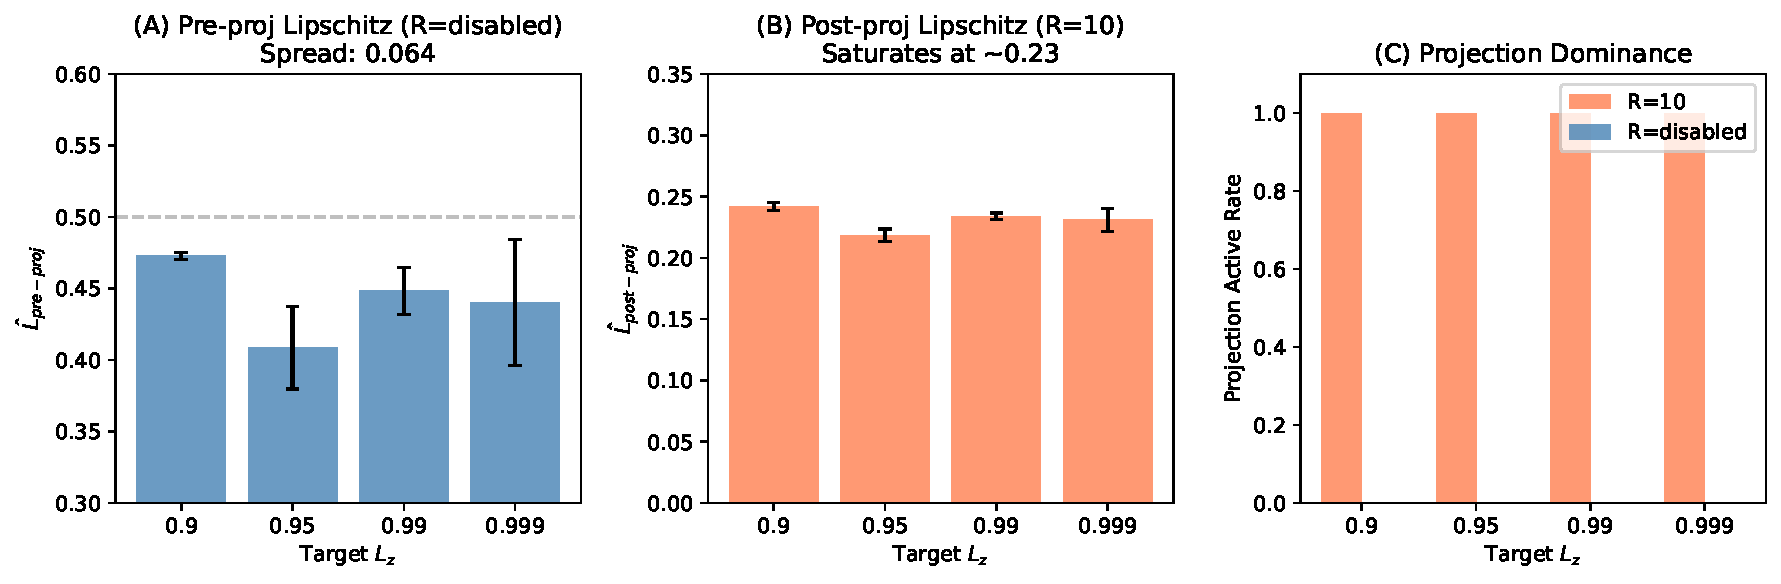
\includegraphics[width=\textwidth]{results/paper_ready/exp2_final/fig_exp2_dial_does_not_control_Lz.pdf}
    \caption{Spectral-norm dial does not control Lipschitz constant. (A) Pre-projection Lipschitz varies weakly across target $L_z$ values. (B) Post-projection Lipschitz saturates at $R=10$. (C) Projection dominates at $R=10$ (100\% active).}
    \label{fig:exp2_dial_failure}
\end{figure}

\begin{figure}[h]
    \centering
    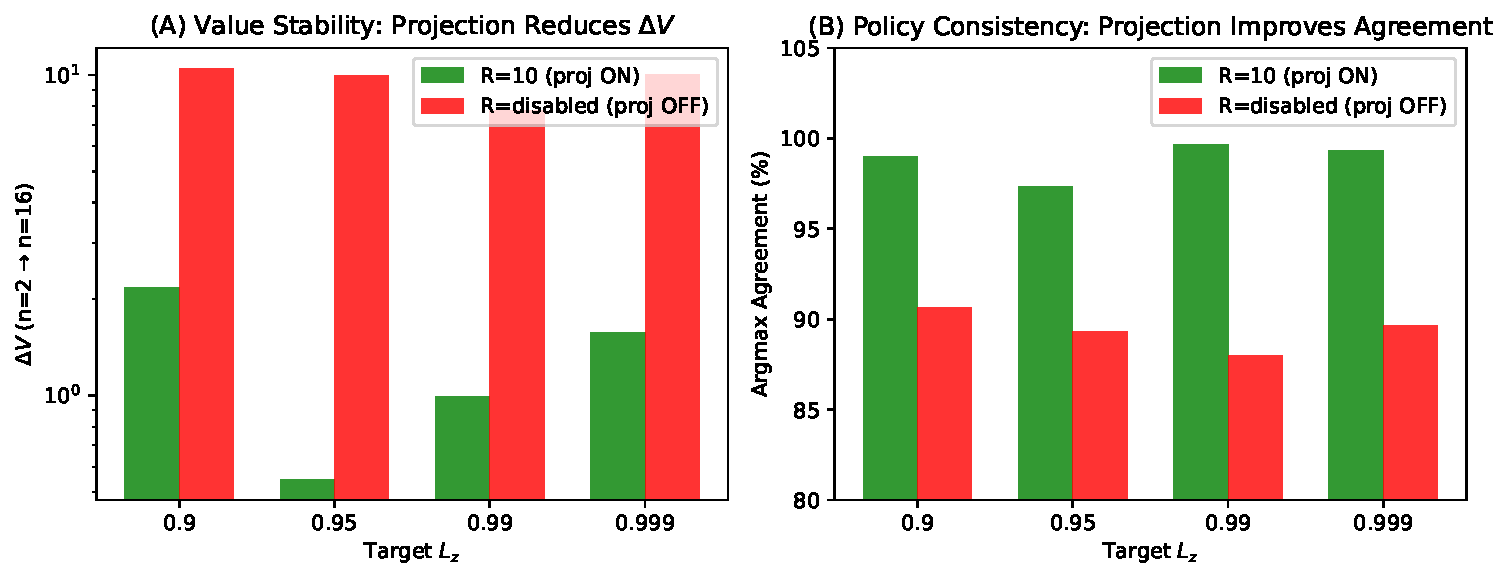
\includegraphics[width=0.8\textwidth]{results/paper_ready/exp2_final/fig_exp2_projection_is_primary_stabilizer.pdf}
    \caption{Projection is the primary stabilizer. (A) $\Delta V$ dramatically reduces with projection enabled. (B) Argmax agreement improves with projection.}
    \label{fig:exp2_projection_stabilizer}
\end{figure}
